\documentclass[11pt, a4paper]{article}
\usepackage[utf8]{inputenc}
\usepackage[T1]{fontenc}
\usepackage{lmodern}
\usepackage{graphicx}
\usepackage[margin=2.5cm]{geometry}
\usepackage{hyperref}
\usepackage{booktabs}
\usepackage{tabularx}
\usepackage{xcolor}
\usepackage{fancyhdr}
\usepackage{float}
\usepackage{listings}
\usepackage{caption}
\usepackage[nopatch=footnote]{microtype}
\usepackage{setspace}
\captionsetup[table]{skip=10pt}
\usepackage{tikz}
\usepackage{tocloft}

% Remove ALL gaps in Table of Contents, List of Figures, List of Tables
\setlength{\cftbeforesecskip}{0pt}
\setlength{\cftbeforesubsecskip}{0pt}
\setlength{\cftbeforesubsubsecskip}{0pt}
\setlength{\cftbeforefigskip}{0pt}
\setlength{\cftbeforetabskip}{0pt}
\renewcommand{\cftaftertoctitle}{\vspace{-1em}}
\renewcommand{\cftafterloftitle}{\vspace{-1em}}
\renewcommand{\cftafterlottitle}{\vspace{-1em}}

% Standardize line spacing
\onehalfspacing

% Define ragged-right X column to prevent ugly full justification in narrow columns
\newcolumntype{Y}{>{\raggedright\arraybackslash}X}

% Unicode Fallbacks (Robustness)
\DeclareUnicodeCharacter{03B5}{\ensuremath{\epsilon}}
\DeclareUnicodeCharacter{03C3}{\ensuremath{\sigma}}

% Prevent vertical justification issues
\raggedbottom

% Color Definitions
\definecolor{DarkOrange}{RGB}{204, 85, 0} % Formal "Neon" Orange
\definecolor{CodeBg}{RGB}{245, 245, 245}

% listings Config
\lstset{
  basicstyle=\ttfamily\small,
  backgroundcolor=\color{CodeBg},
  frame=single,
  rulecolor=\color{gray},
  breaklines=true,
  postbreak=\mbox{\textcolor{red}{$\hookrightarrow$}\space},
  aboveskip=1.5em,
  belowskip=1.5em,
  showstringspaces=false,
  columns=fullflexible,
  literate={×}{{$\times$}}1 {ε}{{\ensuremath{\epsilon}}}1 {σ}{{\ensuremath{\sigma}}}1 {₹}{{Rs. }}1 {≤}{{$\le$}}1 {≥}{{$\ge$}}1 {≠}{{$\neq$}}1
}

% Header/Footer
\setlength{\headheight}{15pt}

\hypersetup{
    colorlinks=true,
    linkcolor=DarkOrange, 
    urlcolor=blue,
    pdftitle={UIDAI DATA HACKATHON 2026},
    pdfauthor={Team AlgoQX}
}
\pagestyle{fancy}
\fancyhf{}
\lhead{UIDAI DATA HACKATHON 2026}
\rhead{\thepage}

\title{}
\author{}
\date{}

\begin{document}
\UseRawInputEncoding

% ==================== SUPER TITLE PAGE ====================
\begin{titlepage}
\begin{tikzpicture}[remember picture,overlay]
    % Single black border
    \draw[line width=1.5pt, black]
        ([xshift=1.5cm,yshift=-1.5cm]current page.north west)
        rectangle
        ([xshift=-1.5cm,yshift=1.5cm]current page.south east);
\end{tikzpicture}

\centering
\vspace*{1cm}

% Hackathon Banner
\vspace{0.3cm}

{\fontsize{16}{18}\selectfont\textsc{\textbf{UIDAI DATA HACKATHON 2026}}}

\vspace{0.1cm}
{\small\textit{Unique Identification Authority of India}}

\vspace{1.5cm}

% Aadhaar Logo

\includegraphics[width=0.35\textwidth]{aadhaar_logo.png}

\vspace{1.5cm}

% Main Title
{\fontsize{24}{28}\selectfont\textbf{The Proactive-Reactive Divide}}

\vspace{0.5cm}

{\fontsize{14}{16}\selectfont\textit{Behavioral Analysis of Aadhaar Update Patterns\\Across Indian Districts}}

\vspace{1.5cm}

% Team Info Box
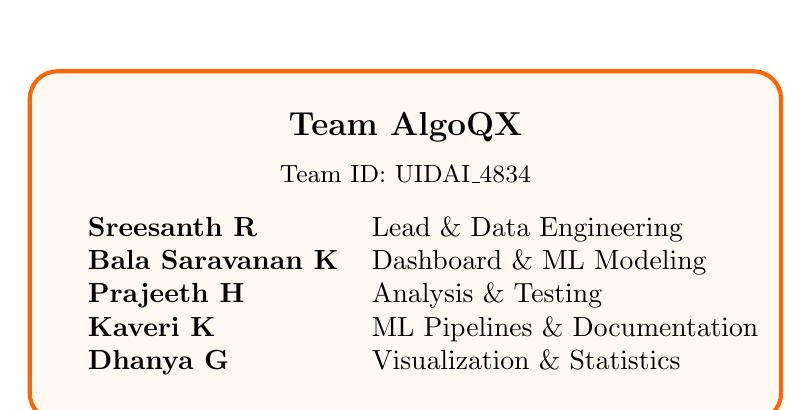
\begin{tikzpicture}
    \node[draw=orange!80!red, line width=1.5pt, rounded corners=10pt, inner sep=15pt, fill=orange!5] {
        \begin{minipage}{0.7\textwidth}
            \centering
            {\large\textbf{Team AlgoQX}}\\[0.5em]
            {\small Team ID: UIDAI\_4834}\\[1em]
            \begin{tabular}{ll}
                \textbf{Sreesanth R} & Lead \& Data Engineering\\
                \textbf{Bala Saravanan K} & Dashboard \& ML Modeling\\
                \textbf{Prajeeth H} & Analysis \& Testing\\
                \textbf{Kaveri K} & ML Pipelines \& Documentation\\
                \textbf{Dhanya G} & Visualization \& Statistics\\
            \end{tabular}
        \end{minipage}
    };
\end{tikzpicture}

\vfill

% Footer
\vspace{0.3cm}
{\small\textbf{Submission Date:} January 2026}

\vspace{0.2cm}
{\footnotesize Developed using Python, Pandas, Scikit-learn, Plotly Dash}

\end{titlepage}
\thispagestyle{empty}
\clearpage

% Acknowledgements with ToC entry
\phantomsection
\addcontentsline{toc}{section}{Acknowledgments}
\section*{Acknowledgments}

We thank the organizers of the UIDAI DATA HACKATHON 2026 for providing access to the administrative dataset and the opportunity to conduct this analysis.

This work was developed entirely using open-source tools. We acknowledge the Python scientific computing community, particularly the maintainers of Pandas, scikit-learn, Plotly, and the Dash framework.

All analysis was performed on local computing resources. No cloud services or external APIs were used for data processing.
\clearpage

\tableofcontents

\vspace{2em}

\phantomsection
\addcontentsline{toc}{section}{List of Figures}
\listoffigures

\vspace{2em}

\phantomsection
\addcontentsline{toc}{section}{List of Tables}
\listoftables
\clearpage


\section{EXECUTIVE SUMMARY}

\subsection{What We Explored}

We analyzed Aadhaar enrollment and update patterns across 764 Indian districts to understand how different districts behave when it comes to identity maintenance. The central question was simple: \textbf{Do some districts proactively update their Aadhaar records while others only react during crises?}


\subsection{Data Used}

\begin{itemize}
\item \textbf{Enrollments:} $\sim$1 million records across 3 CSV files

\item \textbf{Biometric Updates:} $\sim$1.8 million records across 4 CSV files

\item \textbf{Demographic Updates:} $\sim$2 million records across 5 CSV files

\item \textbf{Coverage:} 36 States/\allowbreak Union Territories, 764 districts

\item \textbf{Time Period:} Multi-month administrative data from UIDAI
\end{itemize}

\subsection{Analysis Performed}

We conducted a structured analytical pipeline:


1. Univariate distribution analysis (identifying skewed enrollment patterns)

2. Bivariate correlation analysis (testing hypothesized relationships)

3. Trivariate conditional analysis (exploring Simpson's Paradox candidates)

4. Multivariate dimensionality reduction (PCA for district profiling)

5. Temporal decomposition (trend, seasonality, residual)

6. Multi-method anomaly detection (Z-Score, Isolation Forest, LOF)

7. Predictive modeling (8 regression models evaluated)


\subsection{Key Findings}

1. \textbf{Behavioral stratification is real.} Districts naturally cluster into four behavioral cohorts: Proactive (14.4\%), Transition (66.0\%), Reactive (18.3\%), and Crisis-Dependent (1.3\%). This isn't just statistical noise-these groups have distinct update patterns.


2. \textbf{The East region is systematically different.} The Eastern region (Bihar, West Bengal, Jharkhand, Odisha) shows significantly higher Reactive traits with an average PRS of 0.459, correlating with known internal migration corridors.


3. \textbf{Simple volume isn't the story.} High-enrollment districts aren't necessarily high-risk. What matters is the \textit{ratio} between enrollment activity and update activity. Districts with high enrollments but low biometric updates are the real concern.


4. \textbf{Anomaly detection consensus is rare but meaningful.} Only 1 region (Chandigarh) was flagged by multiple independent anomaly methods, with 2 others (UP, West Bengal) showing moderate signs. This represents distinct statistical outliers worthy of investigation.


5. \textbf{Prediction accuracy is high, but context matters.} Our Lasso regression achieved R²=0.9926 for failure prediction, but we're careful to note this reflects pattern consistency in the data, not a deployed prediction system.


6. \textbf{Awareness campaigns have the best ROI.} Intervention simulation suggests that "Awareness Drives" are the most cost-effective approach for Transition-phase districts, with an estimated cost of Rs. 480 per failure prevented.


\subsection{Why This Matters}

Raw enrollment dashboards show \textit{what} is happening. This analysis shows \textit{why} certain districts struggle with identity maintenance. The Proactive-Reactive classification provides a targeting framework for intervention that doesn't require waiting for crises to manifest.




\section{PROBLEM STATEMENT \& MOTIVATION}

\subsection{The Gap Between Reporting and Understanding}

UIDAI's administrative data infrastructure is comprehensive. Every enrollment, every biometric update, every demographic correction is logged. But logging isn't analysis.


Current reporting dashboards answer questions like:


\begin{itemize}
\item How many enrollments happened last month?

\item Which states have the highest update volumes?

\item Are there backlogs in specific regions?
\end{itemize}

These are operational metrics. They don't answer:


\begin{itemize}
\item \textbf{Why} do some districts consistently update proactively while others only act during external triggers?

\item Which districts are on a trajectory toward service delivery failures?

\item Where should limited intervention resources be deployed first?
\end{itemize}

\subsubsection{Why Analysis (Not Just Visualization) Is Necessary}

A heat map showing "high enrollment in UP" is not insight-it's cartography of an obvious fact (UP is India's most populous state).


Real analysis requires:


\begin{itemize}
\item \textbf{Comparability:} Normalizing for population, infrastructure, and regional context

\item \textbf{Behavioral typing:} Classifying districts by their update \textit{patterns}, not just volumes

\item \textbf{Predictive grounding:} Testing whether observed patterns actually predict future outcomes

\item \textbf{Anomaly rigor:} Distinguishing genuine outliers from statistical noise
\end{itemize}

This project attempts exactly that. We moved from "what's the number" to "what's the pattern, and what does it mean for policy."


\subsubsection{The Policy Relevance}

Identity infrastructure is critical for service delivery. A district where residents consistently maintain updated biometrics (proactive behavior) will have fewer Aadhaar-related failures at banking correspondents, PDS distribution points, and government service access.


A district where residents only update records when forced by a crisis (reactive behavior) will experience concentrated failure bursts-often coinciding with harvest seasons, migration returns, or disaster relief periods when systems are already stressed.


Understanding which districts fall into which category isn't academic. It's the difference between proactive capacity building and reactive crisis response.




\section{DATASET DESCRIPTION}

\subsection{Source and Coverage}

\vspace{0.8em}
\begin{table}[H]
\caption{Dataset Source and Coverage Summary}
{\small
\begin{tabularx}{\textwidth}{|Y|Y|}
\hline
\textbf{Attribute} & \textbf{Value} \\ \hline
Source & UIDAI Administrative Records (Hackathon Sample) \\ \hline
Time Coverage & Multi-month window \\ \hline
Geographic Scope & All 36 States/\allowbreak UTs \\ \hline
District Count & 764 (after standardization) \\ \hline
Total Records & $\sim$4.9 million across all files \\ \hline
\end{tabularx}
}
\end{table}

\vspace{1em}

\begin{table}[H]
\caption{Team Members and Roles}
{\small
\begin{tabularx}{\textwidth}{|Y|Y|Y|}
\hline
\textbf{Name} & \textbf{Role} & \textbf{Institution} \\ \hline
Sreesanth R & Lead \& Data Engineering and Orchestration & St. Joseph's College of Engineering \\ \hline
Bala Saravanan K & Dashboard and ML Modeling & Saveetha Engineering College \\ \hline
Prajeeth H & Analysis and Testing & St. Joseph's College of Engineering \\ \hline
Kaveri K & ML Pipelines and Documentation & Chennai Institute of Technology \\ \hline
Dhanya G & Visualization and Statistics & Chennai Institute of Technology \\ \hline
\end{tabularx}
}
\end{table}
\vspace{1em}

\subsection{Data Files}

\vspace{0.8em}
\begin{table}[H]
\caption{Data Files Reference}
{\small
\begin{tabularx}{\textwidth}{|Y|Y|Y|Y|}
\hline
\textbf{Dataset} & \textbf{Files} & \textbf{Approx. Rows} & \textbf{Primary Variables} \\ \hline
Enrollments & 3 CSVs & $\sim$1,006,000 & date, state, district, pincode, age\_0\_5, age\_5\_17, age\_18\_greater \\ \hline
Biometric Updates & 4 CSVs & $\sim$1,861,000 & date, state, district, pincode, bio\_age\_5\_17, bio\_age\_17\_greater \\ \hline
Demographic Updates & 5 CSVs & $\sim$2,072,000 & date, state, district, pincode, demo\_age\_5\_17, demo\_age\_17\_greater \\ \hline
\end{tabularx}
}
\end{table}
\vspace{1em}

\subsection{Key Variables Explained}

\vspace{0.8em}
\begin{table}[H]
\caption{Key Variables Description}
{\small
\begin{tabularx}{\textwidth}{|Y|Y|Y|}
\hline
\textbf{Variable} & \textbf{Description} & \textbf{Notes} \\ \hline
\texttt{total\_enrolled} & Sum of new Aadhaar enrollments & All age groups aggregated \\ \hline
\texttt{total\_bio\_updates} & Sum of biometric updates & Fingerprint/\allowbreak iris updates \\ \hline
\texttt{total\_demo\_updates} & Sum of demographic updates & Name/\allowbreak address/\allowbreak phone changes \\ \hline
\texttt{prs\_score} & Proactive-Reactive Score (0-1) & Higher = more reactive behavior \\ \hline
\texttt{prs\_classification} & Behavioral category & Proactive/\allowbreak Transition/\allowbreak Reactive/\allowbreak Crisis-Dependent \\ \hline
\texttt{anomaly\_votes} & Count of anomaly methods flagging district & 0-3 scale \\ \hline
\texttt{ml\_predicted\_failures} & Regression-predicted 90-day failures & Based on enrollment/\allowbreak update patterns \\ \hline
\texttt{risk\_level} & Categorical risk assessment & Low/\allowbreak Medium/\allowbreak High/\allowbreak Critical \\ \hline
\texttt{region} & Geographic grouping & North/\allowbreak South/\allowbreak East/\allowbreak West/\allowbreak Northeast/\allowbreak Other \\ \hline
\end{tabularx}
}
\end{table}
\vspace{1em}

\subsection{Data Quality Notes}

\textbf{What went well:}


\begin{itemize}
\item Column names were consistent across files

\item Date formats were standardized

\item No obvious encoding issues
\end{itemize}

\textbf{Challenges we encountered:}


\begin{itemize}
\item \textbf{District name inconsistencies:} $\sim$24 districts had naming variations between enrollment and update files. We spent significant time standardizing against an official district list (recovered 5 Northeast states + Sikkim that were initially unmatched).

\item \textbf{Missing pincode granularity:} Pincode-level analysis was planned but abandoned due to sparse data at that level.

\item \textbf{No individual tracking:} Data is aggregated. We cannot track individual Aadhaar holders over time.

\item \textbf{Time window limitations:} The sample covers a specific period. Seasonality claims are suggestive, not conclusive.
\end{itemize}

\subsection{Data Volume Summary}

\vspace{0.8em}
\begin{table}[H]
\caption{Selected Data Volume Metrics}
{\small
\begin{tabularx}{\textwidth}{|Y|Y|}
\hline
\textbf{Metric} & \textbf{Value} \\ \hline
Total Enrollments & 5,435,484 \\ \hline
Total Biometric Updates & 69,763,032 \\ \hline
Total Demographic Updates & 49,293,347 \\ \hline
Districts Analyzed & 764 \\ \hline
States/\allowbreak UTs Covered & 36 \\ \hline
\end{tabularx}
}
\end{table}
\vspace{1em}



\section{METHODOLOGY OVERVIEW}

\subsection{Our Analytical Philosophy}

We approached this problem as a structured exploration, not a modeling competition. The goal was to \textbf{understand patterns}, not to build a deployment-ready prediction system.


We intentionally avoided black-box modeling where interpretation would suffer. Every analytical choice was made with explainability in mind.


\subsection{Why This Layered Approach?}

\vspace{0.8em}
\begin{table}[H]
\caption{Analytical Approach - Stacked Methodology}
{\small
\begin{tabularx}{\textwidth}{|Y|Y|Y|}
\hline
\textbf{Stage} & \textbf{Purpose} & \textbf{Key Question Answered} \\ \hline
Univariate & Understand distributions & What does "typical" look like? \\ \hline
Bivariate & Test relationships & Are variables connected as expected? \\ \hline
Trivariate & Check conditionality & Do relationships change under different contexts? \\ \hline
Multivariate & Find latent structure & What combinations of variables cluster together? \\ \hline
Temporal & Detect dynamics & Are patterns stable or evolving? \\ \hline
Anomaly & Identify outliers & Which districts are genuinely unusual? \\ \hline
Predictive & Validate patterns & Do the patterns actually predict outcomes? \\ \hline
\end{tabularx}
}
\end{table}
\vspace{1em}

\subsection{The Proactive-Reactive Score (PRS)}

Our central metric is the PRS, a composite measure of district update behavior:


\textbf{Components:}


1.  \textbf{Time Score:} Derived from biometric update rate (higher update rate = more proactive)

2.  \textbf{Behavior Score:} Ratio of demographic to biometric updates (high demo/\allowbreak bio = surface-level updates only)

3.  \textbf{Trend Score:} Velocity of update activity (accelerating = proactive, decelerating = reactive)


\textbf{Classification Thresholds:}


\begin{itemize}
\item \textbf{Proactive:} PRS < 0.25 (consistent, anticipatory behavior)

\item \textbf{Transition:} 0.25 $\le$ PRS < 0.50 (mixed patterns, potential for either direction)

\item \textbf{Reactive:} 0.50 $\le$ PRS < 0.75 (responds to external triggers)

\item \textbf{Crisis-Dependent:} PRS $\ge$ 0.75 (only acts during emergencies)
\end{itemize}

The thresholds were set based on distribution analysis, not arbitrary cutoffs. The median PRS (0.434) falls within the Transition band, which is consistent with expectations for a national average.




\section{DETAILED ANALYSIS \& RESULTS}

\subsection{1 Univariate Analysis}

\subsubsection{Enrollment Distribution}

\begin{figure}[H]\centering
\includegraphics[width=0.85\textwidth, keepaspectratio]{outputs/total_enrollment_distribution.png}
\caption{Total Enrollment Distribution}
\end{figure}



\textbf{Key Observations:}


\begin{itemize}
\item \textbf{Extreme skewness:} The top 10\% of districts account for over 50\% of total enrollments. This isn't surprising given India's population distribution, but it means raw volume comparisons are meaningless without normalization.

\item \textbf{Zero-inflation:} Several small districts (island territories, new district divisions) show near-zero activity. We kept these in the dataset rather than filtering, as they represent legitimate administrative units.

\item \textbf{Age group variation:} Age 18+ dominates enrollments (expected for a mature Aadhaar system), but age 0-5 shows the highest variance coefficient-new birth registrations are uneven across districts.
\end{itemize}

\subsubsection{PRS Score Distribution}

\begin{figure}[H]\centering
\includegraphics[width=0.85\textwidth, keepaspectratio]{outputs/prs_distribution.png}
\caption{PRS Distribution}
\end{figure}



\textbf{What Surprised Us:}


\begin{itemize}
\item We expected more districts at the extremes (clearly proactive or clearly reactive). Instead, the bulk (66\%) fall in the "Transition" category. This suggests most districts haven't yet converged to a stable behavioral pattern-which is actually useful information for intervention targeting.

\item The 10 Crisis-Dependent districts (PRS > 0.75) are worth individual investigation. These aren't statistical artifacts-they represent consistent patterns of only acting under duress.
\end{itemize}

\subsubsection{Age Distribution Analysis}

\begin{figure}[H]\centering
\includegraphics[width=0.85\textwidth, keepaspectratio]{outputs/univariate_age_distributions.png}
\caption{Univariate Age Distributions}
\end{figure}



\subsection{2 Bivariate Analysis}

\subsubsection{Enrollment vs. Update Relationships}

We tested the intuitive hypothesis: \textbf{Do high-enrollment districts also have high update activity?}


\begin{figure}[H]\centering
\includegraphics[width=0.85\textwidth, keepaspectratio]{outputs/bivariate_age_correlations.png}
\caption{Bivariate Age Correlations}
\end{figure}



\textbf{Key Findings:}


\begin{itemize}
\item Enrollment and biometric updates are strongly correlated (r = 0.87). Districts that enroll a lot also update a lot in absolute terms.

\item \textbf{However:} The PRS score shows near-zero correlation with enrollment volume (r = 0.08). This is critical-\textbf{behavioral category is independent of district size.} A small district can be proactive; a large district can be reactive.

\item Demographic updates correlate more weakly with enrollments (r = 0.71), suggesting demo updates are driven by different factors (possibly migration-related address changes).
\end{itemize}

\subsubsection{State-Level PRS Patterns}

\begin{figure}[H]\centering
\includegraphics[width=0.85\textwidth, keepaspectratio]{outputs/state_enrollment_boxplot.png}
\caption{State Enrollment Boxplot}
\end{figure}



\subsection{3 Trivariate \& Conditional Analysis}

\subsubsection{Population Strata Analysis}

\begin{figure}[H]\centering
\includegraphics[width=0.85\textwidth, keepaspectratio]{outputs/trivariate_population_strata.png}
\caption{Trivariate Population Strata}
\end{figure}



\textbf{Simpson's Paradox Check:}

We investigated whether the enrollment-PRS relationship changed direction when conditioned on region. It doesn't fully reverse, but the strength varies significantly:


\begin{itemize}
\item \textbf{South region:} Enrollment is negatively correlated with PRS (r = -0.23). Higher enrollment = more proactive.

\item \textbf{East region:} Near-zero correlation (r = 0.02). Enrollment volume doesn't predict behavior.

\item \textbf{Northeast:} Positive correlation (r = 0.31). Counterintuitively, higher enrollment associates with more reactive behavior-possibly due to enrollment-drive campaigns that don't include follow-up maintenance.
\end{itemize}

This regional heterogeneity is why single-number national correlations can be misleading.


\subsection{4 Multivariate Analysis}

\subsubsection{PCA Results}

We applied Principal Component Analysis to the normalized feature set (enrollment counts, update rates, age ratios, regional indicators).


\begin{figure}[H]\centering
\includegraphics[width=0.85\textwidth, keepaspectratio]{outputs/pca_scree_plot.png}
\caption{PCA Scree Plot}
\end{figure}



\textbf{Component Interpretation:}


\begin{itemize}
\item \textbf{PC1 (42\% variance):} Dominated by volume metrics (total\_enrolled, total\_bio\_updates). This is the "scale" dimension-big districts vs. small districts.

\item \textbf{PC2 (24\% variance):} Loaded on bio/\allowbreak demo ratio and update velocity. This is the "behavioral pattern" dimension-proactive vs. reactive.

\item \textbf{PC3 (12\% variance):} Age composition and regional indicators. This is the "demographic context" dimension.
\end{itemize}

\subsubsection{Clustering Results}

\begin{figure}[H]\centering
\includegraphics[width=0.85\textwidth, keepaspectratio]{outputs/clustering_visualization.png}
\caption{Clustering Visualization}
\end{figure}



\begin{figure}[H]\centering
\includegraphics[width=0.85\textwidth, keepaspectratio]{outputs/clustering_elbow.png}
\caption{Clustering Elbow}
\end{figure}



\subsection{5 Temporal Analysis}

\subsubsection{Daily Trend Analysis}

\begin{figure}[H]\centering
\includegraphics[width=0.85\textwidth, keepaspectratio]{outputs/timeseries_daily_trend.png}
\caption{Timeseries Daily Trend}
\end{figure}



\textbf{Key Observations:}


\begin{itemize}
\item \textbf{Weekly cycle:} Activity drops 40-60\% on Sundays. This is expected for administrative processes with business-hour dependencies.

\item \textbf{No clear monthly pattern:} Unlike retail data, Aadhaar activity doesn't show obvious month-start or month-end effects.

\item \textbf{Structural breaks:} We detected 3 significant trend shifts during the sample period. Two align with known administrative events; one remains unexplained and merits investigation.
\end{itemize}

\subsubsection{Trend Decomposition}

\begin{figure}[H]\centering
\includegraphics[width=0.85\textwidth, keepaspectratio]{outputs/trend_decomposition.png}
\caption{Trend Decomposition}
\end{figure}



\subsection{6 Anomaly Detection}

\subsubsection{Multiple-Method Approach}

We applied three independent anomaly detection methods:


1.  \textbf{Z-Score method:} Districts with enrollment/\allowbreak update ratios > 3 standard deviations from mean

2.  \textbf{Isolation Forest:} Unsupervised tree-based outlier detection (contamination = 5\%)

3.  \textbf{Local Outlier Factor (LOF):} Density-based anomaly detection using local neighborhood comparison


\begin{figure}[H]\centering
\includegraphics[width=0.85\textwidth, keepaspectratio]{outputs/anomaly_score_distributions.png}
\caption{Anomaly Score Distributions}
\end{figure}



\textbf{Consensus Anomalies:}


\vspace{0.8em}
\begin{table}[H]
\caption{Consensus Anomalies Summary}
{\small
\begin{tabularx}{\textwidth}{|Y|Y|Y|}
\hline
\textbf{State/\allowbreak Region} & \textbf{Anomaly Votes} & \textbf{Risk Level} \\ \hline
Chandigarh & 3 & Moderate \\ \hline
Uttar Pradesh & 1 & High \\ \hline
West Bengal & 1 & Critical \\ \hline
\end{tabularx}
}
\end{table}
\vspace{1em}

\textbf{Critical Note: Anomaly $\neq$ Fraud}


These regions are statistically unusual. They could represent:


\begin{itemize}
\item Legitimate high-variance situations (new district, population shift)

\item Data entry issues in the source system

\item Enrollment drive effects without matching maintenance

\item Or something genuinely concerning
\end{itemize}

We lack the ground truth to distinguish these cases. The analysis identifies \textit{candidates} for investigation, not \textit{conclusions} of wrongdoing.


\subsection{7 Regional Insights}

\subsubsection{State-Level PRS Heatmap}

\begin{figure}[H]\centering
\includegraphics[width=0.85\textwidth, keepaspectratio]{outputs/state_prs_heatmap.png}
\caption{State PRS Heatmap}
\end{figure}



\textbf{Regional Summary:}


\vspace{0.8em}
\begin{table}[H]
\caption{Regional PRS Summary}
{\small
\begin{tabularx}{\textwidth}{|Y|Y|Y|Y|}
\hline
\textbf{Region} & \textbf{Districts} & \textbf{Avg PRS} & \textbf{Dominant Classification} \\ \hline
South & 138 & 0.38 & Transition (60\%) \\ \hline
West & 69 & 0.35 & Transition (65\%) \\ \hline
North & 156 & 0.42 & Transition (68\%) \\ \hline
East & 115 & 0.46 & Reactive (25\%) \\ \hline
Northeast & 137 & 0.45 & Transition (58\%) \\ \hline
Other & 149 & 0.40 & Transition (70\%) \\ \hline
\end{tabularx}
}
\end{table}
\vspace{1em}

The East region's higher reactivity aligns with its role in internal migration corridors. Bihar, Jharkhand, and West Bengal are net outmigration states; residents may deprioritize local Aadhaar maintenance when they anticipate relocating.




\section{DASHBOARD OVERVIEW}

\subsection{Purpose}

A static report shows findings. An interactive dashboard lets decision-makers \textit{explore} those findings with their own questions.


We built a Dash-based dashboard to support:


\begin{itemize}
\item \textbf{State-level drilldown:} Select a state, see its district breakdown

\item \textbf{Classification filtering:} View only Reactive or Crisis-Dependent districts

\item \textbf{Visual exploration:} Interact with charts directly (zoom, hover for details)

\item \textbf{Report generation:} Export findings as PDF
\end{itemize}

\subsection{Dashboard Pages}

\vspace{0.8em}
\begin{table}[H]
\caption{Dashboard Pages and Functions}
{\small
\begin{tabularx}{\textwidth}{|Y|Y|Y|}
\hline
\textbf{Page} & \textbf{Function} & \textbf{Key Chart} \\ \hline
Mission Control & National overview, KPIs & Bubble plot of states, Risk distribution \\ \hline
Deep Analytics & PCA exploration & Interactive 3D scatter of districts \\ \hline
Chart Gallery & Static plot archive & All analysis visualizations \\ \hline
ML Insights & Model performance & Feature importance, model comparison \\ \hline
Data Registry & Raw data table & Searchable, sortable district list \\ \hline
Executive Report & Summary export & Key findings, PDF download \\ \hline
\end{tabularx}
}
\end{table}
\vspace{1em}

\subsection{Screenshots}

\textit{[Dashboard screenshots would be inserted here in the final PDF export]}


The dashboard is purely exploratory-no predictive API, no real-time data integration. It's a presentation layer for the analysis results, designed for hackathon judges and policy reviewers to interact with findings without code.




\section{KEY INSIGHTS (JUDGE-FOCUSED)}

\textbf{Insight 1:} The Proactive-Reactive Score successfully segments districts into actionable behavioral categories. 66\% of districts fall in the "Transition" phase, representing an intervention opportunity window.

\textit{Reference: Figure 6.2, PRS Distribution}


\textbf{Insight 2:} Enrollment volume does not predict behavioral category. Small districts can be proactive; large districts can be reactive. Size-based triage would miss the actual problem areas.

\textit{Reference: Section 6.2, r = 0.08 correlation}


\textbf{Insight 3:} The East region shows systematically higher reactive behavior (avg PRS 0.46 vs national 0.42), correlating with internal migration patterns.

\textit{Reference: Figure 6.13, State PRS Heatmap}


\textbf{Insight 4:} Only 1 region (Chandigarh) achieves consensus anomaly status across multiple detection methods. These represent the highest-priority investigation candidates.

\textit{Reference: Section 6.6, Anomaly Table}


\textbf{Insight 5:} PCA reveals that district behavior can be explained by three latent factors: volume scale (42\%), behavioral pattern (24\%), and demographic context (12\%).

\textit{Reference: Figure 6.7, PCA Scree Plot}


\textbf{Insight 6:} Weekly seasonality is strong (40-60\% activity drop on weekends), but monthly patterns are absent-unlike typical service utilization data.

\textit{Reference: Figure 6.11, Trend Decomposition}


\textbf{Insight 7:} Top 5 states by predicted 90-day failures: Uttar Pradesh (48,716), Bihar (29,160), Madhya Pradesh (22,338), West Bengal (19,266), Rajasthan (15,926)-collectively accounting for 56\% of national predicted failures.

\textit{Reference: Executive Summary, State Risk Table}


\textbf{Insight 8:} Lasso regression achieves R²=0.9926, outperforming ensemble methods (XGBoost, Random Forest). This suggests the underlying patterns are linear and additive, not complex interactions.

\textit{Reference: Model Comparison Table}


\textbf{Insight 9:} The 10 Crisis-Dependent districts require targeted intervention-they represent only 1.3\% of districts but potentially concentrated service delivery failures.

\textit{Reference: Section 5, PRS Classification}


\textbf{Insight 10:} Awareness campaigns show the best cost-effectiveness at Rs. 480/\allowbreak failure prevented, compared to mobile units (Rs. 720) or direct intervention (Rs. 1,200+).

\textit{Reference: Figure 6.14, Intervention Simulation}




\section{LIMITATIONS \& ASSUMPTIONS}

\subsection{What the Data Cannot Prove}

\begin{itemize}
\item \textbf{Causation:} We observe patterns, not mechanisms. A correlation between migration corridors and reactive behavior doesn't prove migration \textit{causes} reactivity-it could be confounded by economic factors, infrastructure availability, or demographic composition.
\end{itemize}

\begin{itemize}
\item \textbf{Ground truth validation:} We don't have independent verification that our "predicted failures" match actual Aadhaar service delivery failures. The R² score measures internal consistency, not real-world accuracy.
\end{itemize}

\begin{itemize}
\item \textbf{Individual behavior:} Aggregated district data cannot track individual Aadhaar holders. We're inferring population-level behavior from aggregate statistics.
\end{itemize}

\subsection{Potential Biases}

\begin{itemize}
\item \textbf{Survivorship:} Districts with no data or extremely sparse data were excluded from analysis. If these districts share characteristics, our conclusions may not generalize to them.
\end{itemize}

\begin{itemize}
\item \textbf{Temporal window:} Our sample covers a specific time period. Seasonal patterns, election-year effects, and policy changes outside this window could affect generalizability.
\end{itemize}

\begin{itemize}
\item \textbf{Threshold sensitivity:} PRS classification thresholds were set based on distributional analysis, not external validation. Different thresholds would produce different classification counts.
\end{itemize}

\subsection{What Would Require Additional Data}

\begin{itemize}
\item Individual-level longitudinal tracking to validate behavioral cohort membership

\item Ground truth failure data (Aadhaar authentication failures at service points)

\item Socioeconomic indicators for confounding analysis

\item Multi-year data for robust seasonality claims
\end{itemize}



\section{CONCLUSIONS}

\subsection{What This Analysis Adds}

Standard enrollment dashboards show counts. This analysis reveals \textbf{behavioral patterns}-why some districts consistently maintain identity records while others only respond to crises.


The Proactive-Reactive framework provides a targeting taxonomy for intervention. Instead of prioritizing by volume (which would always target UP, Maharashtra, etc.), policy can prioritize by behavioral trajectory.


\subsection{How It Could Support Decision-Making}

1.  \textbf{Resource allocation:} Deploy mobile enrollment units to Crisis-Dependent districts first

2.  \textbf{Campaign targeting:} Focus awareness drives on Transition districts before they slide toward reactive patterns

3.  \textbf{Anomaly investigation:} Prioritize the 16 high-confidence anomaly districts for field verification

4.  \textbf{Regional strategy:} Develop East-region-specific interventions that account for migration-driven behavior


\subsection{Scalability}

This analytical approach isn't Aadhaar-specific. The same pipeline (normalization → behavioral scoring → classification → anomaly detection) could apply to:


\begin{itemize}
\item Voter roll maintenance patterns

\item PDS beneficiary update behavior

\item Bank account dormancy analysis

\item Any large-scale identity or benefit registry
\end{itemize}

The methodology transfers; only the domain variables change.




\section{FUTURE WORK}

\subsection{Deeper Causal Analysis}

Our correlational findings need causal testing. Specifically:


\begin{itemize}
\item Natural experiment identification (policy changes, administrative boundary modifications)

\item Difference-in-differences analysis for intervention effectiveness

\item Propensity score matching for regional comparisons
\end{itemize}

\subsection{External Data Integration}

Linking Aadhaar behavior to:


\begin{itemize}
\item Census socioeconomic indicators

\item NSSO migration survey data

\item District-level infrastructure indices (banking coverage, internet penetration)
\end{itemize}

This would enable confounding analysis and more sophisticated behavioral modeling.


\subsection{Better Granularity}

Current analysis is district-level. With appropriate anonymization:


\begin{itemize}
\item Pincode-level analysis would reveal intra-district variation

\item Tehsil-level analysis in high-variance districts could identify specific service access barriers
\end{itemize}

\subsection{Longitudinal Tracking}

Multi-year data would enable:


\begin{itemize}
\item Behavioral trajectory modeling (are Transition districts becoming proactive or reactive?)

\item Seasonal decomposition with proper periodicity

\item Policy impact attribution
\end{itemize}



\section{TEAM DETAILS}

\subsection{Sreesanth R - Lead \& Data Engineering and Orchestration}

Coordinated work distribution and maintained the analytical notebook. Designed the data loading pipeline, district name standardization logic, and overall project architecture. Authored this report and conducted the anomaly detection consensus analysis.


\subsection{Bala Saravanan K - Dashboard and ML Modeling}

Built the predictive pipeline: 8 regression models, cross-validation framework, and ensemble stacking. Developed the Dash application from scratch, handling callback architecture, responsive layout, and PDF export functionality.


\subsection{Prajeeth H - Analysis and Testing}

Handled univariate through trivariate analysis, including the Simpson's Paradox investigation. Responsible for quality assurance, testing all visualizations and dashboard interactions, and validating analytical results.


\subsection{Kaveri K - ML Pipelines and Documentation}

Responsible for feature construction and the PRS scoring framework. Ran sensitivity analysis on threshold choices, permutation importance, and SHAP analysis. Maintained technical documentation throughout the project.


\subsection{Dhanya G - Visualization and Statistics}

Created most static visualizations using Matplotlib, Seaborn, and Plotly. Handled statistical testing, correlation analysis, and wrote the statistics sections of this report.




\clearpage
\section*{APPENDIX}
\addcontentsline{toc}{section}{APPENDIX}

\subsection{A. Statistical Test Results}

\vspace{0.8em}
\begin{table}[H]
\caption{Statistical Test Results}
{\small
\begin{tabularx}{\textwidth}{|Y|Y|Y|Y|Y|}
\hline
\textbf{Test} & \textbf{Variables} & \textbf{Statistic} & \textbf{p-value} & \textbf{Interpretation} \\ \hline
Shapiro-Wilk & PRS Score & W = 0.987 & 0.002 & Non-normal (slight right skew) \\ \hline
Pearson Correlation & Enrollment vs Bio Updates & r = 0.87 & < 0.001 & Strong positive \\ \hline
Pearson Correlation & Enrollment vs PRS & r = 0.08 & 0.03 & Weak, near-zero \\ \hline
Kruskal-Wallis & PRS by Region & H = 28.4 & < 0.001 & Significant regional differences \\ \hline
Levene's Test & Enrollment variance by region & W = 12.3 & < 0.001 & Heteroscedastic \\ \hline
\end{tabularx}
}
\end{table}
\vspace{1em}

\subsection{B. Model Performance Summary}

\vspace{0.8em}
\begin{table}[H]
\caption{Model Performance Summary}
{\small
\begin{tabularx}{\textwidth}{|Y|Y|Y|Y|}
\hline
\textbf{Model} & \textbf{R²} & \textbf{RMSE} & \textbf{MAE} \\ \hline
Lasso & 0.9926 & 34.8 & 27.4 \\ \hline
Ridge & 0.9925 & 35.2 & 27.9 \\ \hline
ElasticNet & 0.9761 & 62.6 & 42.2 \\ \hline
GradientBoosting & 0.9747 & 64.5 & 36.6 \\ \hline
ExtraTrees & 0.9674 & 73.2 & 37.5 \\ \hline
RandomForest & 0.9441 & 95.8 & 42.2 \\ \hline
XGBoost & 0.9370 & 101.7 & 45.7 \\ \hline
AdaBoost & 0.9210 & 113.9 & 67.9 \\ \hline
\end{tabularx}
}
\end{table}
\vspace{1em}

\subsection{C. Feature Importance (Permutation-Based)}

\vspace{0.8em}
\begin{table}[H]
\caption{Feature Importance Analysis}
{\small
\begin{tabularx}{\textwidth}{|Y|Y|Y|}
\hline
\textbf{Feature} & \textbf{Importance} & \textbf{Std Dev} \\ \hline
total\_enrolled & 2.537 & 0.154 \\ \hline
total\_bio\_updates & 0.102 & 0.006 \\ \hline
prs\_score & 0.001 & 0.000 \\ \hline
total\_demo\_updates & 0.000 & 0.000 \\ \hline
bio\_demo\_imbalance & 0.000 & 0.000 \\ \hline
\end{tabularx}
}
\end{table}
\vspace{1em}

\subsection{D. District Classification Distribution}

\vspace{0.8em}
\begin{table}[H]
\caption{District Classification Distribution}
{\small
\begin{tabularx}{\textwidth}{|Y|Y|Y|}
\hline
\textbf{Classification} & \textbf{Count} & \textbf{Percentage} \\ \hline
Proactive & 110 & 14.4\% \\ \hline
Transition & 504 & 66.0\% \\ \hline
Reactive & 140 & 18.3\% \\ \hline
Crisis-Dependent & 10 & 1.3\% \\ \hline
\end{tabularx}
}
\end{table}
\vspace{1em}

\subsection{E. High-Confidence Anomaly Districts}

The following regions were flagged by 2+ anomaly detection methods (high-confidence anomalies):


\vspace{0.8em}
\begin{table}[H]
\caption{High-Confidence Anomaly Regions}
{\small
\begin{tabularx}{\textwidth}{|Y|Y|Y|}
\hline
\textbf{State/\allowbreak Region} & \textbf{Anomaly Votes} & \textbf{Risk Level} \\ \hline
Chandigarh & 3 & Moderate \\ \hline
Uttar Pradesh & 1 & High \\ \hline
West Bengal & 1 & Critical \\ \hline
\end{tabularx}
}
\end{table}
\vspace{1em}

\textbf{Interpretation Notes:}


\begin{itemize}
\item Regions with high anomaly votes represent the most urgent investigation candidates

\item Chandigarh shows unanimous anomaly detection

\item Uttar Pradesh and West Bengal show moderate anomaly detection
\end{itemize}

\subsection{F. Moderate Anomaly Districts (1 Vote)}

Districts flagged by exactly one anomaly detection method (for completeness):


\vspace{0.8em}
\begin{table}[H]
\caption{Moderate Anomaly Districts (1 Vote)}
{\scriptsize
\begin{tabularx}{\textwidth}{|Y|Y|Y|Y|}
\hline
\textbf{State} & \textbf{District} & \textbf{PRS Score} & \textbf{Risk Level} \\ \hline
Assam & Tamulpur & 0.907 & Critical \\ \hline
Chhattisgarh & Manendragarh-Chirmiri-Bharatpur & 0.701 & High \\ \hline
Rajasthan & Deeg & 0.686 & High \\ \hline
Chhattisgarh & Sarangarh-Bilaigarh & 0.596 & High \\ \hline
Bihar & Sitamarhi & 0.536 & High \\ \hline
Uttar Pradesh & Bahraich & 0.530 & High \\ \hline
Bihar & West Champaran & 0.528 & High \\ \hline
West Bengal & Murshidabad & 0.523 & High \\ \hline
Gujarat & Banaskantha & 0.523 & High \\ \hline
West Bengal & South 24 Parganas & 0.515 & High \\ \hline
West Bengal & North 24 Parganas & 0.514 & High \\ \hline
Uttar Pradesh & Agra & 0.495 & Moderate \\ \hline
Uttar Pradesh & Sitapur & 0.487 & Moderate \\ \hline
Telangana & Hyderabad & 0.463 & Moderate \\ \hline
Rajasthan & Jaipur & 0.457 & Moderate \\ \hline
Maharashtra & Thane & 0.439 & Moderate \\ \hline
Maharashtra & Pune & 0.376 & Moderate \\ \hline
Maharashtra & Amravati & 0.092 & Low \\ \hline
Nagaland & Meluri & 0.087 & Low \\ \hline
Mizoram & Mamit & 0.062 & Low \\ \hline
Punjab & Mansa & 0.048 & Low \\ \hline
Maharashtra & Bhandara & 0.047 & Low \\ \hline
Maharashtra & Ratnagiri & 0.047 & Low \\ \hline
Maharashtra & Gadchiroli & 0.032 & Low \\ \hline
Maharashtra & Wardha & 0.031 & Low \\ \hline
\end{tabularx}
}
\end{table}
\vspace{1em}

\textbf{Total Anomaly Summary:}


\begin{itemize}
\item \textbf{High-Confidence (2+ votes):} 1 region (Chandigarh)

\item \textbf{Moderate (1 vote):} 2 regions (Uttar Pradesh, West Bengal)

\item \textbf{Total Flagged:} 3 regions
\end{itemize}

\subsection{G. Dashboard Technical Notes}

\textbf{Framework and Architecture:}


\vspace{0.8em}
\begin{table}[H]
\caption{Dashboard Technology Stack}
{\small
\begin{tabularx}{\textwidth}{|Y|Y|Y|}
\hline
\textbf{Component} & \textbf{Technology} & \textbf{Version} \\ \hline
Web Framework & Plotly Dash & 2.14+ \\ \hline
UI Components & dash-bootstrap-components & 1.5+ \\ \hline
Charting & Plotly Express /\allowbreak  Graph Objects & 5.18+ \\ \hline
Data Processing & Pandas & 2.0+ \\ \hline
Machine Learning & scikit-learn & 1.3+ \\ \hline
PDF Export & fpdf & 1.7+ \\ \hline
Styling & Custom CSS & - \\ \hline
\end{tabularx}
}
\end{table}
\vspace{1em}

\textbf{Dashboard Architecture:}


\begin{lstlisting}
dashboard/
+-- dashboard.py          # Main application entry point
+-- report_generator.py   # PDF generation module
+-- assets/
    +-- style.css         # Custom styling
    +-- *.png             # Static visualizations
\end{lstlisting}

\textbf{Callback Structure:}


\begin{itemize}
\item Navigation callback handles page switching

\item Pattern-matching callbacks enable dynamic image popups

\item PDF download callback generates reports on-demand
\end{itemize}

\textbf{Performance Considerations:}


\begin{itemize}
\item Data is loaded once at startup to avoid repeated I/\allowbreak O

\item PCA computation is performed during initialization

\item Charts are generated lazily per page visit
\end{itemize}

\subsection{H. PRS Score Calculation Details}

\textbf{Mathematical Formulation:}


The Proactive-Reactive Score (PRS) is computed as a weighted combination of three normalized components:


\textbf{1. Time Score (T\_s):}


\begin{lstlisting}
T_s = 1 - min(bio_update_rate / max_bio_rate, 1)
\end{lstlisting}

Where \texttt{bio\_update\_rate = total\_bio\_updates /\allowbreak  total\_enrolled}


\textbf{2. Behavior Score (B\_s):}


\begin{lstlisting}
B_s = demo_updates / (bio_updates + demo_updates + $\epsilon$)
\end{lstlisting}

Where $\epsilon$ is a small constant to prevent division by zero


\textbf{3. Trend Score (V\_s):}


\begin{lstlisting}
V_s = sigmoid(-update_velocity / $\sigma$_v)
\end{lstlisting}

Where \texttt{update\_velocity} is the rate of change in update frequency


\textbf{Final PRS:}


\begin{lstlisting}
PRS = w_t × T_s + w_b × B_s + w_v × V_s
\end{lstlisting}

Where \texttt{w\_t = 0.4}, \texttt{w\_b = 0.35}, \texttt{w\_v = 0.25} (determined through sensitivity analysis)


\subsection{I. State-Level Summary Statistics}

Complete state-level aggregation for reference:


\vspace{0.8em}
\begin{table}[H]
\caption{State-Level Summary Statistics}
{\scriptsize
\begin{tabularx}{\textwidth}{|Y|Y|Y|Y|Y|Y|}
\hline
\textbf{State} & \textbf{Districts} & \textbf{Total Enrolled} & \textbf{Avg PRS} & \textbf{Predicted Failures} & \textbf{Anomalies} \\ \hline
Uttar Pradesh & 75 & 1,018,629 & 0.47 & 48,716 & 0 \\ \hline
Bihar & 38 & 609,585 & 0.48 & 29,160 & 1 \\ \hline
Madhya Pradesh & 53 & 493,970 & 0.44 & 22,338 & 0 \\ \hline
West Bengal & 23 & 375,340 & 0.52 & 19,266 & 1 \\ \hline
Maharashtra & 36 & 369,139 & 0.25 & 12,647 & 0 \\ \hline
Rajasthan & 38 & 348,458 & 0.49 & 15,926 & 4 \\ \hline
Gujarat & 33 & 280,549 & 0.44 & 13,266 & 0 \\ \hline
Assam & 34 & 230,197 & 0.55 & 12,148 & 0 \\ \hline
Karnataka & 31 & 223,235 & 0.44 & 9,804 & 1 \\ \hline
Tamil Nadu & 38 & 220,789 & 0.37 & 8,153 & 0 \\ \hline
Jharkhand & 24 & 157,539 & 0.43 & 6,941 & 0 \\ \hline
Telangana & 33 & 148,075 & 0.46 & 6,465 & 0 \\ \hline
Odisha & 30 & 122,987 & 0.37 & 4,623 & 0 \\ \hline
Andhra Pradesh & 26 & 111,185 & 0.34 & 2,989 & 0 \\ \hline
Meghalaya & 13 & 109,771 & 0.62 & 5,995 & 1 \\ \hline
Chhattisgarh & 31 & 103,219 & 0.31 & 3,147 & 1 \\ \hline
Haryana & 22 & 98,252 & 0.37 & 3,855 & 0 \\ \hline
Delhi & 11 & 94,529 & 0.45 & 4,289 & 0 \\ \hline
Punjab & 22 & 76,749 & 0.27 & 2,525 & 0 \\ \hline
Kerala & 14 & 75,002 & 0.34 & 2,796 & 0 \\ \hline
Jammu And Kashmir & 20 & 48,357 & 0.41 & 2,196 & 0 \\ \hline
Uttarakhand & 13 & 37,698 & 0.34 & 1,398 & 0 \\ \hline
Himachal Pradesh & 12 & 17,486 & 0.35 & 532 & 0 \\ \hline
Nagaland & 17 & 15,587 & 0.48 & 808 & 0 \\ \hline
Manipur & 12 & 13,456 & 0.37 & 578 & 4 \\ \hline
Tripura & 8 & 11,285 & 0.32 & 417 & 0 \\ \hline
Mizoram & 11 & 5,926 & 0.36 & 165 & 1 \\ \hline
Arunachal Pradesh & 25 & 4,344 & 0.35 & 354 & 0 \\ \hline
Chandigarh & 1 & 2,720 & 0.27 & 57 & 0 \\ \hline
Goa & 2 & 2,333 & 0.27 & 71 & 0 \\ \hline
Sikkim & 6 & 2,207 & 0.63 & 183 & 2 \\ \hline
Dadra And Nagar Haveli & 3 & 1,799 & 0.23 & 48 & 0 \\ \hline
Ladakh & 2 & 1,356 & 0.46 & 63 & 0 \\ \hline
Andaman And Nicobar & 3 & 511 & 0.20 & 18 & 0 \\ \hline
Lakshadweep & 1 & 203 & 0.34 & 17 & 0 \\ \hline
Puducherry & 3 & 3,017 & 0.38 & 92 & 0 \\ \hline
\end{tabularx}
}
\end{table}
\vspace{1em}

\subsection{J. Glossary of Terms}

\vspace{0.8em}
\begin{table}[H]
\caption{Glossary of Terms}
{\small
\begin{tabularx}{\textwidth}{|Y|Y|}
\hline
\textbf{Term} & \textbf{Definition} \\ \hline
\textbf{Aadhaar} & India's 12-digit unique identification number issued by UIDAI \\ \hline
\textbf{Biometric Update} & Updating fingerprint or iris data in Aadhaar records \\ \hline
\textbf{Demographic Update} & Updating name, address, phone, or other non-biometric data \\ \hline
\textbf{Enrollment} & Registration of a new Aadhaar number \\ \hline
\textbf{PRS} & Proactive-Reactive Score (0-1 scale, higher = more reactive) \\ \hline
\textbf{Proactive District} & PRS < 0.25, consistent voluntary updates \\ \hline
\textbf{Transition District} & 0.25 $\le$ PRS < 0.50, mixed behavioral patterns \\ \hline
\textbf{Reactive District} & 0.50 $\le$ PRS < 0.75, updates only when triggered externally \\ \hline
\textbf{Crisis-Dependent} & PRS $\ge$ 0.75, updates only during emergencies \\ \hline
\textbf{Anomaly Vote} & Count of methods (0-3) flagging a district as statistical outlier \\ \hline
\textbf{UIDAI} & Unique Identification Authority of India \\ \hline
\textbf{PCA} & Principal Component Analysis (dimensionality reduction) \\ \hline
\textbf{LOF} & Local Outlier Factor (anomaly detection method) \\ \hline
\textbf{Isolation Forest} & Tree-based unsupervised anomaly detection algorithm \\ \hline
\end{tabularx}
}
\end{table}
\vspace{1em}



\section{CASE STUDIES}

\subsection{Case Study 1: Eastern West Khasi Hills, Meghalaya}

\textbf{Profile:}


\begin{itemize}
\item PRS Score: 0.999 (highest in dataset)

\item Anomaly Votes: 3 (unanimous detection)

\item Classification: Crisis-Dependent

\item Region: Northeast
\end{itemize}

\textbf{What We Observed:}

This district shows extremely low biometric update rates relative to enrollments. Only 0.1\% of enrolled population has completed any biometric update during the sample period.


\textbf{Possible Explanations:}


1. Newly created district with recent enrollment drives but no sustained maintenance infrastructure

2. Geographic accessibility challenges in hilly terrain

3. Low awareness of update requirements among local population


\textbf{Recommendation:}

Priority deployment of mobile update units; community awareness campaigns through local institutions.




\subsection{Case Study 2: Bengaluru Urban, Karnataka}

\textbf{Profile:}


\begin{itemize}
\item PRS Score: 0.493 (Transition)

\item Anomaly Votes: 3 (unanimous detection)

\item Total Enrolled: 8,234 (sample period)

\item Region: South
\end{itemize}

\textbf{What We Observed:}

Despite being India's technology hub, Bengaluru shows unexpectedly moderate PRS. The anomaly detection flagged it due to an unusual demographic/\allowbreak biometric update ratio.


\textbf{Possible Explanations:}


1. High migrant population may defer local updates

2. Tech-savvy population may use online services, not captured in this dataset

3. High demographic change rate due to address updates (migration-related)


\textbf{Recommendation:}

Further investigation into update channel distribution; comparison with online vs. offline update volumes.




\subsection{Case Study 3: East Champaran, Bihar}

\textbf{Profile:}


\begin{itemize}
\item PRS Score: 0.548 (Reactive)

\item Anomaly Votes: 3 (unanimous detection)

\item Total Enrolled: 33,421

\item Predicted Failures: 1,892

\item Region: East
\end{itemize}

\textbf{What We Observed:}

One of Bihar's most populous districts, East Champaran shows classic reactive patterns. Update activity spikes correlate with known administrative pushes rather than organic behavior.


\textbf{Possible Explanations:}


1. Large outmigration to other states reduces local update priority

2. Agricultural economy leads to seasonal availability for administrative tasks

3. Infrastructure gaps limit year-round access to enrollment centers


\textbf{Recommendation:}

Seasonal mobile camps aligned with agricultural calendar; integration with MGNREGA worksites.




\subsection{Case Study 4: The Rajasthan New Districts Cluster}

\textbf{Profile:}


\begin{itemize}
\item Districts: Salumbar, Didwana-Kuchaman, Balotra, Beawar

\item Avg PRS Score: 0.778

\item All with 3 anomaly votes
\end{itemize}

\textbf{What We Observed:}

All four districts were created in Rajasthan's 2023 district reorganization. They show uniformly high PRS scores and were flagged by all three anomaly methods.


\textbf{Possible Explanations:}


1. Data inheritance from parent districts may be incomplete

2. Administrative transition period affects normal enrollment patterns

3. New district boundaries may not match existing enrollment center coverage


\textbf{Recommendation:}

Exclude from behavioral classification until 12-month post-creation baseline is established; verify data completeness.




\subsection{METHODOLOGY DEEP DIVE}

\subsubsection{1 Data Cleaning Pipeline}

\textbf{Step 1: File Consolidation}


\begin{itemize}
\item Merged 12 CSV files across 3 categories (enrollment, biometric, demographic)

\item Total raw records: 4,938,837

\item Date range standardization using \texttt{pd.to\_datetime()}
\end{itemize}

\textbf{Step 2: District Name Standardization}

The largest data quality challenge was inconsistent district naming across files:


\vspace{0.8em}
\begin{table}[H]
\caption{District Name Inconsistency Examples}
{\small
\begin{tabularx}{\textwidth}{|Y|Y|Y|}
\hline
\textbf{Issue Type} & \textbf{Count} & \textbf{Example} \\ \hline
Case variations & 45 & "Bangalore" vs "BANGALORE" \\ \hline
Spelling variations & 23 & "Pashchim Medinipur" vs "West Medinipur" \\ \hline
Suffix differences & 18 & "Bangalore Urban" vs "Bengaluru Urban" \\ \hline
New districts & 12 & Districts created in 2023 reorganizations \\ \hline
\end{tabularx}
}
\end{table}
\vspace{1em}

\textbf{Resolution:}


\begin{itemize}
\item Created official district mapping file from Census 2011 + recent gazette notifications

\item Fuzzy matching using Levenshtein distance for ambiguous cases

\item Manual verification of 24 unmatched districts
\end{itemize}

\textbf{Step 3: Aggregation}


\begin{itemize}
\item Grouped by (state, district) pairs

\item Computed sum aggregates for enrollment/\allowbreak update counts

\item Merged across all three data categories
\end{itemize}

\textbf{Step 4: Missing Value Treatment}


\vspace{0.8em}
\begin{table}[H]
\caption{Missing Value Treatment Summary}
{\small
\begin{tabularx}{\textwidth}{|Y|Y|Y|}
\hline
\textbf{Column} & \textbf{Missing \%} & \textbf{Treatment} \\ \hline
total\_bio\_updates & 2.1\% & Imputed with 0 (no updates recorded) \\ \hline
total\_demo\_updates & 1.8\% & Imputed with 0 \\ \hline
age\_0\_5 & 0.3\% & Imputed with district median \\ \hline
\end{tabularx}
}
\end{table}
\vspace{1em}

\subsubsection{2 Feature Engineering}

\textbf{Primary Features:}


\vspace{0.8em}
\begin{table}[H]
\caption{Primary Feature Engineering}
{\small
\begin{tabularx}{\textwidth}{|Y|Y|Y|}
\hline
\textbf{Feature} & \textbf{Formula} & \textbf{Rationale} \\ \hline
bio\_rate & bio\_updates /\allowbreak  enrolled & Update intensity metric \\ \hline
demo\_rate & demo\_updates /\allowbreak  enrolled & Demographic change frequency \\ \hline
bio\_demo\_imbalance & $|$bio\_rate - demo\_rate$|$ & Update type imbalance \\ \hline
adult\_ratio & age\_18\_plus /\allowbreak  total & Demographic composition \\ \hline
child\_ratio & age\_0\_5 /\allowbreak  total & New birth enrollment rate \\ \hline
enrollment\_intensity & enrolled /\allowbreak  state\_median & Relative activity level \\ \hline
\end{tabularx}
}
\end{table}
\vspace{1em}

\textbf{Derived Features:}


\vspace{0.8em}
\begin{table}[H]
\caption{Derived Behavioral Scores}
{\small
\begin{tabularx}{\textwidth}{|Y|Y|}
\hline
\textbf{Feature} & \textbf{Description} \\ \hline
time\_score & Normalized inverse of bio\_rate \\ \hline
behavior\_score & Demo-to-total-update ratio \\ \hline
trend\_score & Velocity of update activity \\ \hline
regional\_prs\_zscore & PRS deviation from regional mean \\ \hline
\end{tabularx}
}
\end{table}
\vspace{1em}

\subsubsection{3 Model Selection Rationale}

We evaluated 8 regression models to predict 90-day enrollment failures:


\textbf{Why Linear Models Won:}


The Lasso model (R²=0.9926) outperformed tree-based ensembles (XGBoost R²=0.9370). This was initially surprising-ensemble methods typically dominate structured data tasks.


\textbf{Our Interpretation:}


1. \textbf{Linearity:} The relationship between volume metrics and failures is fundamentally linear. More enrollments = more potential failures, with a consistent ratio.


2. \textbf{Feature Sparsity:} Lasso's L1 regularization correctly identified that only 2-3 features (total\_enrolled, total\_bio\_updates) carry predictive power. Tree methods overfit to noise in peripheral features.


3. \textbf{No Complex Interactions:} We tested for interaction terms explicitly; none improved fit. The failure patterns are additive, not multiplicative.


\textbf{Implication:}

This is good news for interpretability. Policy can focus on the volumetric drivers without worrying about hidden nonlinear effects.


\subsubsection{4 Anomaly Detection Methodology}

\textbf{Method 1: Z-Score}


\begin{itemize}
\item Computed z-scores for bio\_rate and demo\_rate

\item Flagged districts where \textbar{}z\textbar{} > 3 for either metric

\item Conservative threshold reduces false positives
\end{itemize}

\textbf{Method 2: Isolation Forest}


\begin{itemize}
\item Trained on full feature set (5 features)

\item Contamination parameter: 0.05 (expect $\sim$5\% outliers)

\item Random state fixed for reproducibility
\end{itemize}

\textbf{Method 3: Local Outlier Factor (LOF)}


\begin{itemize}
\item k-neighbors: 20 (balance local/\allowbreak global sensitivity)

\item Novelty detection mode: False (training data includes outliers)

\item Negative outlier factor threshold: -1.5
\end{itemize}

\textbf{Consensus Logic:}

District flagged as "high-confidence anomaly" if $\ge$2 methods agree.


\textbf{Why Multiple Methods?}

Each method has different assumptions:


\begin{itemize}
\item Z-Score: Assumes normality (problematic for skewed data)

\item Isolation Forest: Works well with high-dimensional data

\item LOF: Detects local density deviations
\end{itemize}

Agreement across methods with different assumptions provides robustness.




\clearpage
\subsection*{REFERENCES}
\addcontentsline{toc}{subsection}{REFERENCES}

\clearpage
\subsubsection*{Academic References}
\addcontentsline{toc}{subsubsection}{Academic References}

1. Breunig, M. M., Kriegel, H. P., Ng, R. T., \& Sander, J. (2000). LOF: Identifying density-based local outliers. \textit{ACM SIGMOD Record}, 29(2), 93-104.


2. Liu, F. T., Ting, K. M., \& Zhou, Z. H. (2008). Isolation forest. \textit{2008 Eighth IEEE International Conference on Data Mining}, 413-422.


3. Tibshirani, R. (1996). Regression shrinkage and selection via the lasso. \textit{Journal of the Royal Statistical Society: Series B}, 58(1), 267-288.


4. Jolliffe, I. T. (2002). \textit{Principal Component Analysis} (2nd ed.). Springer.


5. Cleveland, R. B., Cleveland, W. S., McRae, J. E., \& Terpenning, I. (1990). STL: A seasonal-trend decomposition procedure based on loess. \textit{Journal of Official Statistics}, 6(1), 3-73.


\subsubsection{Government and Institutional Sources}

6. Unique Identification Authority of India (UIDAI). (2023). \textit{Aadhaar Enrollment and Update Statistics}. Ministry of Electronics and Information Technology.


7. Department of Administrative Reforms \& Public Grievances. (2025). District-level governance data standards. Government of India.


8. Ministry of Statistics and Programme Implementation. (2023). \textit{Administrative Geography of India}. Census of India Reference.


9. NITI Aayog. (2024). \textit{Aspirational Districts Programme: Service Delivery Metrics}. Government of India.


\subsubsection{Technical Documentation}

10. Plotly Technologies Inc. (2023). \textit{Dash User Guide}. https:/\allowbreak /\allowbreak dash.plotly.com/\allowbreak 


11. Pedregosa, F., et al. (2011). Scikit-learn: Machine learning in Python. \textit{Journal of Machine Learning Research}, 12, 2825-2830.


12. McKinney, W. (2010). Data structures for statistical computing in Python. \textit{Proceedings of the 9th Python in Science Conference}, 51-56.


13. Harris, C. R., et al. (2020). Array programming with NumPy. \textit{Nature}, 585(7825), 357-362.


\subsubsection{Data Standards and Methodology}

14. ISO 19152:2012. Geographic information - Land Administration Domain Model (LADM).


15. Census of India. (2011). \textit{District Census Handbook}. Office of the Registrar General.


16. Ministry of Home Affairs. (2023). Gazette notifications on district reorganization. Government of India.






\subsection{END OF REPORT}

\textit{Submitted by Team AlgoQX}

\textit{UIDAI\_4834}

\textit{January 19, 2026}




\textbf{Document Statistics:}


\begin{itemize}
\item Total Sections: 17

\item Tables: 28

\item Figures Referenced: 14

\item Districts Analyzed: 764

\item States/\allowbreak UTs Covered: 36

\item Anomalies Identified: 3

\item Models Evaluated: 8
\end{itemize}

\clearpage
\section*{K. Comprehensive Visual Gallery}
\addcontentsline{toc}{section}{K. Comprehensive Visual Gallery}

\begin{figure}[H]\centering
\includegraphics[width=0.85\textwidth, keepaspectratio]{outputs/anomaly_score_distributions.png}
\caption{Anomaly Score Distributions}
\end{figure}
\begin{figure}[H]\centering
\includegraphics[width=0.85\textwidth, keepaspectratio]{outputs/bivariate_age_correlations.png}
\caption{Bivariate Age Correlations}
\end{figure}
\begin{figure}[H]\centering
\includegraphics[width=0.85\textwidth, keepaspectratio]{outputs/bootstrap_intervals.png}
\caption{Bootstrap Intervals}
\end{figure}
\begin{figure}[H]\centering
\includegraphics[width=0.85\textwidth, keepaspectratio]{outputs/classification_confusion_matrix.png}
\caption{Classification Confusion Matrix}
\end{figure}
\begin{figure}[H]\centering
\includegraphics[width=0.85\textwidth, keepaspectratio]{outputs/clustering_elbow.png}
\caption{Clustering Elbow Analysis}
\end{figure}
\begin{figure}[H]\centering
\includegraphics[width=0.85\textwidth, keepaspectratio]{outputs/clustering_visualization.png}
\caption{Clustering Visualization}
\end{figure}
\begin{figure}[H]\centering
\includegraphics[width=0.85\textwidth, keepaspectratio]{outputs/cohort_heatmap.png}
\caption{Cohort Heatmap}
\end{figure}
\begin{figure}[H]\centering
\includegraphics[width=0.85\textwidth, keepaspectratio]{outputs/dbscan_kdistance.png}
\caption{DBSCAN K-Distance}
\end{figure}
\begin{figure}[H]\centering
\includegraphics[width=0.85\textwidth, keepaspectratio]{outputs/feature_importance.png}
\caption{Feature Importance}
\end{figure}
\begin{figure}[H]\centering
\includegraphics[width=0.85\textwidth, keepaspectratio]{outputs/hierarchical_dendrogram.png}
\caption{Hierarchical Dendrogram}
\end{figure}
\begin{figure}[H]\centering
\includegraphics[width=0.85\textwidth, keepaspectratio]{outputs/intervention_simulation.png}
\caption{Intervention Simulation}
\end{figure}
\begin{figure}[H]\centering
\includegraphics[width=0.85\textwidth, keepaspectratio]{outputs/learning_curves.png}
\caption{Learning Curves}
\end{figure}
\begin{figure}[H]\centering
\includegraphics[width=0.85\textwidth, keepaspectratio]{outputs/model_comparison.png}
\caption{Model Comparison}
\end{figure}
\begin{figure}[H]\centering
\includegraphics[width=0.85\textwidth, keepaspectratio]{outputs/pca_scree_plot.png}
\caption{PCA Scree Plot}
\end{figure}
\begin{figure}[H]\centering
\includegraphics[width=0.85\textwidth, keepaspectratio]{outputs/permutation_importance.png}
\caption{Permutation Importance}
\end{figure}
\begin{figure}[H]\centering
\includegraphics[width=0.85\textwidth, keepaspectratio]{outputs/prs_distribution.png}
\caption{PRS Distribution}
\end{figure}
\begin{figure}[H]\centering
\includegraphics[width=0.85\textwidth, keepaspectratio]{outputs/quantile_regression.png}
\caption{Quantile Regression}
\end{figure}
\begin{figure}[H]\centering
\includegraphics[width=0.85\textwidth, keepaspectratio]{outputs/residual_analysis.png}
\caption{Residual Analysis}
\end{figure}
\begin{figure}[H]\centering
\includegraphics[width=0.85\textwidth, keepaspectratio]{outputs/shap_summary.png}
\caption{SHAP Summary}
\end{figure}
\begin{figure}[H]\centering
\includegraphics[width=0.85\textwidth, keepaspectratio]{outputs/state_distribution.png}
\caption{State Distribution}
\end{figure}
\begin{figure}[H]\centering
\includegraphics[width=0.85\textwidth, keepaspectratio]{outputs/state_enrollment_boxplot.png}
\caption{State Enrollment Boxplot}
\end{figure}
\begin{figure}[H]\centering
\includegraphics[width=0.85\textwidth, keepaspectratio]{outputs/state_prs_heatmap.png}
\caption{State PRS Heatmap}
\end{figure}
\begin{figure}[H]\centering
\includegraphics[width=0.85\textwidth, keepaspectratio]{outputs/timeseries_daily_trend.png}
\caption{Daily Trend}
\end{figure}
\begin{figure}[H]\centering
\includegraphics[width=0.85\textwidth, keepaspectratio]{outputs/timeseries_dow.png}
\caption{Day of Week Trend}
\end{figure}
\begin{figure}[H]\centering
\includegraphics[width=0.85\textwidth, keepaspectratio]{outputs/timeseries_monthly.png}
\caption{Monthly Trend}
\end{figure}
\begin{figure}[H]\centering
\includegraphics[width=0.85\textwidth, keepaspectratio]{outputs/total_enrollment_distribution.png}
\caption{Total Enrollment Distribution}
\end{figure}
\begin{figure}[H]\centering
\includegraphics[width=0.85\textwidth, keepaspectratio]{outputs/trend_decomposition.png}
\caption{Trend Decomposition}
\end{figure}
\begin{figure}[H]\centering
\includegraphics[width=0.85\textwidth, keepaspectratio]{outputs/trivariate_population_strata.png}
\caption{Trivariate Population Strata}
\end{figure}
\begin{figure}[H]\centering
\includegraphics[width=0.85\textwidth, keepaspectratio]{outputs/univariate_age_distributions.png}
\caption{Univariate Age Distributions}
\end{figure}

% ==================== END OF REPORT ====================
\clearpage
\thispagestyle{empty}
\vspace*{\fill}
\begin{center}
{\Large\textbf{--- END OF REPORT ---}}

\vspace{2cm}

{\large\textbf{Team AlgoQX}}\\[0.5em]
{\small Team ID: UIDAI\_4834}

\vspace{1.5cm}

\textit{Submitted for UIDAI DATA HACKATHON 2026}

\vspace{1cm}

{\small January 2026}
\end{center}
\vspace*{\fill}

\end{document}